%!TEX root = ../thesis.tex
%*******************************************************************************
%****************************** Fourth Chapter **********************************
%*******************************************************************************
\chapter{Age-Related Behavioural Shifts in Flanged Male Orangutans: Insights from Female Association Behaviour and Long Call Patterns}

Primates exhibit a wide range of age-related shifts in social and mating behaviour. Currently, age-related behavioural changes over the lifetime of male orangutans focus primarily on the shifts between the unflanged and flanged morph, and behavioural shifts in ageing flanged male orangutans remain under-researched. Building on previous findings linking age to flange deformation, this study sought to further examine the behavioural changes associated with ageing in these primates, particularly focusing on female association behaviour and long call patterns. This study examined six males from the date of their first long call observed to investigate changes in female associative behaviour and long call composition over time. My results indicate that older flanged males tend to have fewer hours of association with females and produce shorter long calls with fewer pulses. These behavioural trends in older flanged males align with observations in other ageing great apes which show an increase in solitude with age. However, the underlying reasons for this change, whether it is reduced attractiveness or a self-imposed choice, remain undetermined. Preliminary data also imply that younger flanged males might exhibit varied responses to certain long call triggers, potentially indicating an effort to establish territorial dominance. However, this behaviour may also be driven by increasing energetic costs for producing lengthy long calls in older males. This research offers initial insights into the potential reclusiveness of older flanged males and emphasises the importance of factoring in the approximate transition date from unflanged to flanged in future studies on long call behaviours.
   
\section{Introduction}

\subsection{Effects of ageing in primates}

The ageing process in primates is characterised by a number of physiological and physical changes that can have significant impacts on an individual's overall health and reproductive success \citep{Holloszy.2000}. Older individuals experience a gradual decrease in muscle mass and bone density, as these conditions limit mobility and strength they ultimately impact dominance, mating success and survival \citep{Lowenstine.2016, Almeling.2017}.  Decreases in bone density have been observed in ageing captive rhesus macaques, with a gradual decrease in bone density observed in both sexes \citep{Black.2001}. Furthermore, the skin undergoes alterations such as loss of elasticity, leading to wrinkles and slower wound healing \citep{Montagna.1972, Thomas.2001}. Visible changes related to age, such as alterations in skin condition or hair colour, can differ between sexes in their perceptibility and social implications, potentially influencing mate selection and rivalry. For example, \citet{Jolly.2009} found that adult ring-tailed lemur (\textit{Lemur catta}) coat condition deteriorated as the breeding season progressed and these effects were exaggerated in older individuals. 

In addition to these physical alterations, ageing is interlinked with changes in hormonal composition. For example, there is often a reduction in the production of growth hormones, contributing to the observed decreases in muscle mass and bone density \citep{Fischer.2011}. For example, female rhesus macaques show decreased levels of growth hormone (GH) compared to younger individuals \citep{Woller.2002}. Male primates exhibit a gradual decline in testosterone levels that is linked to a decrease in testes volume \citep{HANDELSMAN.1985, Strum.1991}. In males, this decrease in circulating testosterone further impacts muscle mass, bone density, and sexual drive \citep{Zohdy.2014, Kenny.2000}. Age-related declines in testosterone can also affect mental faculties, for example, in humans a decrease in testosterone levels during ageing has been associated with a decrease in visuo-spatial reasoning in men, and supplementation with testosterone increased performance levels \citep{Martin.2007}. Ageing can also alter the production and regulation of cortisol, affecting an individual's stress response, immunity, and metabolic processes \citep{Goncharova.2002}.  Ageing also presents specific challenges to fertility. Although male primates continue to produce sperm throughout their lives, sperm quality and quantity declines with old age, reducing fertility \citep{Sitzmann.2008}. However, female primates can undergo a cessation of ovulation defined as menopause \citep{Walker.2008}. The timing of this event in the life of individuals vary according to species, with some species such as macaques (\textit{Macaca spp.}) and humans undergoing menopause during mid-life, while other species experience much later, such as chimpanzees who appear to experience at the end of their life \citep{Herndon.2012}.  

In addition to these physical impacts, ageing appears to have significant impacts on sociality in primates. As individuals grow older, they can experience a decrease in the size of their social network and the amount of time spent in association with others \citep{Almeling.2017, González.2023}. In female rhesus macaques, older individuals selectively decrease the size of their social network without reducing the amount of time spent socialising, focusing on previous partners and kin \citep{Siracusa.2022}. Similarly, in Barbary macaques (\textit{Macaca sylvanus}), older females engaged in fewer social interactions, spent less time grooming when they did engage in interactions and maintained a smaller social network \citep{Almeling.2016}. However, this trend is not universal, and there are primates that do not show such decrease when ageing. For example, no notable change in social network size has been observed in male bonnet macaques (\textit{Macaca radiata}) \citep{Silk.1994}. Notably however, the trend towards a shrinking social circle shows sex-specific biases, whereby the socially dominant sex appears to be more likely to increase social interaction during ageing compared to the less dominant sex \citep{Corr.2003,Machanda.2020}. It is important to note that many of these studies focus exclusively on females, in part because males experience a higher mortality rate than females and because many studies have been conducted on female-philopatric species \citep{Machanda.2020}.
However, there are some wider differences between humans and most other primates, ageing humans show a notable positivity bias in their social interactions, while the more common trend in primates is a negativity bias. For example, male bonnet macaques show a decrease in the number of groomings initiated with age, while maintaining similar aggression rates to younger males \citep{Silk.1994}. Psychological studies on humans have found that they exhibit a selective memory bias towards positive events and emotions and prioritise engagements that affirm positive interactions as they age \citep{Carstensen.1999}. Interestingly, parallel findings are observed in one of our closest relatives, chimpanzees. Like humans, ageing chimpanzees appear to exhibit preferences for affiliative interactions, especially with well-acquainted conspecifics, and show a decrease in antagonistic encounters \citep{Rosati.2020}.  These trends are often attributed in part to inherently flexible social systems. This dynamism might enable older individuals to exert greater control over their social environment, associating more often with preferred companions and avoiding potential conflicts \citep{Aureli.2008}. Studies on humans have linked this shift towards positivity in social interactions to our ability to perceive our own limited time and re-organise our lives to prioritise emotional wellbeing over long-term goals, which is known as Socioemotional Selectivity Theory (SST) \citep{Carstensen.1999}. Although this trend is correlative with age, it is primarily driven by our perception of the remaining time and, therefore, is also affected by serious illness or significant life events \citep{Löckenhoff.2004}. However, given this requires significant levels of abstract reasoning about one's own mortality, it is unlikely to be the cause of the observed trend in chimpanzees. As such, alternative hypotheses have been suggested to explain these cross-species trends, noting that humans undergo an increased capacity to regulate emotional reactivity with age \citep{Rosati.2020,Grühn.2016}. However, a cross-species study on this alternative hypothesis has not yet been published.

In males these changes may correlate with impacts of ageing on social dominance, many primates show an inverted-U-shaped dominance curve, where older and younger adults are typically less dominant than "prime-aged" adults \citep{Packer.1979, Smuts.1989, Perlman.2016}. Younger adults are more likely to engage in risky behaviour, including challenging established leaders, while older individuals are generally more averse to risk \citep{Wilson.1985, Haux.2022}. This may be largely due to the increased resource-holding potential of prime-aged adults compared to older ones which combined with the increasing social isolation of elderly individuals and aversion to negative social interactions can lead to a sharp decrease in reproductive success when older. However, this framing removes the impact of female mate choice seen in polygynous or polgynandrous mating systems. For example, \citet{Foerg.1982} found that female black-and-white ruffed lemurs preferred older prime-aged males compared to younger ones, based on their ability to ignore challenges from sub-adult and younger prime males. However, in species with these mating systems,  senescence is experienced more severely by males compared to females, due to a combination of evolutionary and early life factors \citep{Graves.2007}. Species with high levels on intrasexual competition have a higher risk of mortality, which can lead to a reduction in the selection against deleterious mutations which can impact senescence \citep{Williams.1957}. 

\subsection{Sexual strategies and ageing in orangutans}

Orangutans are unique among the primate family in displaying irreversible bimaturism, with both the flanged and unflanged male morphs being able to sire offspring \citep{Knott.2008, Utami.2002km8}. As bimaturism can be arrested by social and psychoendoneurological factors, some unflanged males can sire children from as old as 40 without undergoing this transition \citep{Prasetyo.2021} . Given the dispersed polygynous mating system and female preference for flanged males, we see strong competition between males for access to mates and a significant role of female choice in this environment \citep{Harrison.2007ox}. 

Under these conditions, each morph has a different mating strategy to maximise their number of copulations given their secondary sexual characteristics. The larger of the two, the flanged male, possesses most notably a complex laryngeal sac and cheeks pads, and operate a "call and wait" strategy by emitting distinctive long calls and waiting for females to approach \citep{Utami.2002km8, Kunz.2023}. Interactions between flanged males are almost always antagonistic and can result in serious injury or death to the losing party \citep{Setia.2008}. However, given their semi-social lifestyle, flanged males also indirectly assess competition by use of characteristic long calls \citep{Spillmann.2016}. The call starts with a low rumble and builds up to a crescendo of roars and pulses before ending with a series of gurgles \citep{Spillmann.2010}. These long calls can be heard from up to 1.5km away, however they may only be individually identifiable within a range of 400m \citep{Spillmann.2016}. The role of the flange in this strategy remains unclear. Some suggest that the slightly concave shape of the flange aids the individual in locating the source of other long calls, while others believe it helps to focus the long call in a particular direction \citep{Galdikas.1983,Mitani.1985ak1m}. Current research has not found an association between long call rates and fruit availability, suggesting that they are not costly to make, however, the structure of each long call is context dependent and can be triggered by local cues \citep{Spillmann.2016}. Long calls can occur spontaneously, in response to another long call from a different individual and after pushing over a tree \citep{Delgado.2008}. Females seem able to discern the causes of specific long calls, and move a greater distance towards the source of spontaneously produced long calls, than cued long calls \citep{Spillmann.2016}.  

Females also respond to long calls differently, depending on their habitat. In Suaq Balimbing, female orangutans always move towards the long caller, regardless of their reproductive state, while in Tuanan females move towards long calls only if they do not have dependent offspring \citep{Dunkel.2013, Spillmann.2016}. However, these choices are also mediated by the dominance hierarchy of the local area, in sites with stable dominance hierarchies, females are more likely to be found in the presence of the dominant flanged males, and have longer associations with them compared to non-dominant males \citep{Setia.2008}. After approaching a male, females in association can experience attempts from males to force copulation. This degree of direct sexual coercion is unique among great apes, and given the rates of physical wounding during these encounters is very low, \citet{Knott.2009y9d} argues that these mating attempts are \textit{"direct coercion, and not an indirect means to influence or control future female sexual behavior, as seen in species such as chimpanzees and humans"}. Typically this is framed as an unflanged:flanged dichotomy, that due to female preference for flanged males, unflanged males resort to forced copulation; however, rates of forced copulation vary according to study site and dominance hierarchy \citep{Knott.2008, Knott.2009}. For example, in Suaq Balimbing, the ratio of unflanged males to flanged males is significantly higher, and flanged males employ forced matings significantly less than in Bornean field sites, suggesting that females may be moving towards males as a form of protection against forced matings \citep{Knott.2008}. 

\citet{Knott.2009y9d} also reported that a paper then in preparation found female proceptivity to mating attempts also vary according to the body condition of flanged males at Gunung Palung. Reportedly, males classified as "past-prime" based on their body condition and dimished flange size associated with females significantly less, and females were highly resistive to copulation attempts from them. Additionally, this same paper suggested that males in this condition produced long calls at a lower rate than "prime" males \citep{Knott.2009y9d}. These reported changes in calling behaviour are reinforced by own findings indicating a shift in long call behaviour with diminishing flange width (Chapter 3). Chapter 3 found that the main correlative cause of this condition is increasing age, which is expected to have significant impacts on health particularly in sexually dimorphic species \citep{Beirne.2015}. These age-related changes may then reduce their competitiveness in contests between other flanged males, and reduce the quality of their secondary sexual signals.

Given that long calls have unique patterns that can be used for individual identification, and that females seem to be able to discern the causes behind specific calls, it is possible that the composition or structure of the call is affected by the health of the individual that produces it \citep{Spillmann.2017}. Assuming long calls are not energetically costly, as hypothesised previously, the long call rate is unlikely to be unbiased indicators of fitness, however, we may see impacts on the duration or underlying structure \citep{Zahavi.1975}. It is also possible that the structure of the call remains unchanged, but the female response to long calls is affected and moves a shorter distance towards the call before stopping \citep{Spillmann.2010}.

If these calls are diagnostic of individual body condition, we may also see a shift in mating strategy from ageing flanged males from a "call and wait" strategy to a "silent searching" strategy to avoid antagonistic interactions from flanged males likely to win antagonistic interactions. However, this strategy requires a significant amount of time ranging per day, which flanged males typically do not do and given their increased body size such a shift would require a significant increase in energy intake per day \citep{Prasetyo.2021}. However, if these calls do not contain enough information to diagnose individual fitness, then interaction rates will be similar, but the interactions themselves will be impacted once association has begun. 

In this study, I aim to examine the impacts of old age on orangutan mating and long call behaviour using long-term behavioural data sets. I hypothesise that the previously observed relationship between relative orangutan flange width and age (Chapter 3) will have secondary impacts on mating, and long call behaviours will impact flanged male orangutan mating success as they grow older. I also hypothesise that these impacts will be exaggerated by the self-imposed reduction in sociality experienced by many great apes.

Given the impacts of ageing on sociality and mating success across primates and great apes, and given the high density of flanged males and subsequent unstable dominance hierarchy at the study site; I predict:

\begin{enumerate}
    \item   Older flanged males will enter into fewer female associations per day.

    \item When older flanged males do enter into associations with females, they will be shorter than associations between younger flanged males and females.

    \item Older flanged males will be found in association with fertile females less often than younger flanged males.

    \item Older flanged males will produce long calls more often, but with fewer pulses and for a shorter period of time compared to younger flanged males.
\end{enumerate}


\section{Methods}
\subsection{Study site}
Data was collected at Tuanan Orangutan Research Project (2°09'S, 114°26'E) which is located in the Mawas Reserve in Central Kalimantan, Borneo. Orangutans have been followed daily since 2003 and has one of the highest densities of orangutans in Borneo containing approximately 4.5 individuals/km$^{2}$ \citep{Husson.2008}. The site contains a higher number of flanged males compared to unflanged males with approximately 60\% of male focal follows being conducted on flanged males and has an unstable dominance hierarchy between flanged males \citep{Dunkel.2013}. The study site is located within a low-altitude peat-swamp forest, with a history of anthropogenic disturbance \citep{Gaveau.2014}.


\subsection{Behavioural data}
Behavioural data was collected during daily nest to nest behavioural follows using 2 minute instantaneous focal sampling using an established protocol \citep{OU_methods}. To control for variation in association behaviour over the day, and as orangutans are more likely to be located when in association with other party members, only full day focal follows were included in this analysis (\textit{i.e.} followed from nest to nest). Additionally, the number of observation hours per follow was added as an offset to relevant GLMMs. Individuals were only included if they had been observed in the study site in their unflanged morph, for two key reasons. Firstly, the absolute age of all flanged males at Tuanan is not known, age was encoded as either the number of years since they were first observed or, if they were observed in their unflanged state the number of years since they grew their flanges is known. As unflanged orangutans are significantly more social than flanged males and to avoid systematic biases, I chose to exclude all flanged males where their flanging date is unknown. I then coded the flanged date as the first date for which these individuals produced a long call. These totalled 3,256 of focal follow hours across 6 individuals, collected between 2009 and 2018. 

\begin{figure}
\centering
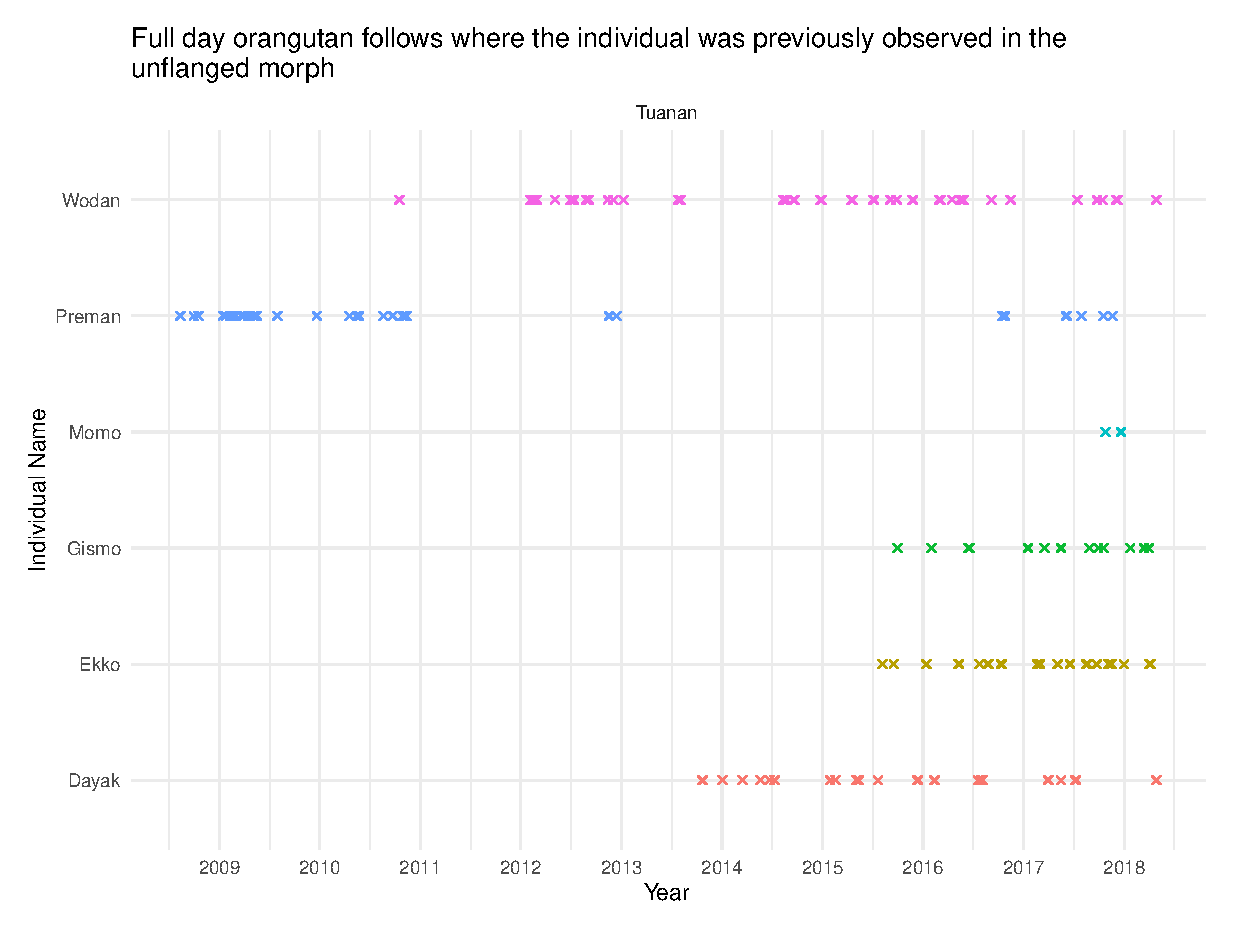
\includegraphics[width=1\linewidth]{Chapter4/Figs/obs_plot.eps}
\caption{Timeline (x-axis) illustrating days where a flanged male previously observed in their unflanged morph was followed for a full follow day at Tuanan Reserach Station. }
\label{fig:Obs_Tuanan_NN}
\end{figure}


\textbf{Association patterns}

Female association patterns were examined by estimating the duration of female association per focal follow day, and the number of females associated with per follow day.  Total female association time was measured as the total number of 2 minute intervals per follow where the focal flanged male was within 50m of a female. Female association time was additive if multiple females were present \textit{e.g.} if two females were present for one 2 minute bout, this would be measured as 4 minutes of female association. The number of females in association per focal follow day was examined using a Poission GLMM, and the total number of female association hours was examined using a Gaussian GLMM. In each model, FAI and relative age were added as fixed effects. As female association can be affected by the number of long calls (LCM) produced by an individual, this was added as a fixed effect for models concerning female association \citep{Spillmann.2010}. As females conceal ovulation and appear to selectively mate according to their fertility, the estimate of female fertility was based on the estimated dates of conception of females \citep{Knott.2009}. Females were coded as likely fertile from one year before estimated conception, or 3 months before the first swelling appears. Only one copulation was observed in our sample, so no copulation analysis has been conducted.

\textbf{Long call patterns}

Long call rates per follow-day and long call pulses per long call were modelled using Poisson GLMMs, and long call duration was modelled using a Gaussian GLMM. As long calls are context dependent and can be used as a form of confrontational assessment, the number of long calls made by other non-focal flanged males that were heard by the observers was included as a term in these analyses \citep{Spillmann.2016}. As long as call behaviour is affected by proximity to females, the number of hours spent within 50m of a female was used a fixed effect \citep{Spillmann.2010}. As association rates are impacted by fruit availability, an interactive effect between FAI and female association was added to our long call models; however, these were not found to be statistically significant, so were removed from our outputs. Additionally, rainfall can have a significant impact on primate calling behaviour; total daily rainfall was included as a term in all long call models (Chapter 3). Finally, relative age, fruit availability, and an interactive term between female association and fruit availability were added as fixed effects. 

\subsection{Ecological data}
Phenological data on fruit availability was taken monthly at both sites throughout the entire study period. The Fruit Availability Index (FAI) was calculated as the percentage of trees with fruits across all surveyed trees (approximately 1000) in the study site. 

\subsection{Analysis}

GLMM analysis was performed using the R version 4.3.0 using the \textit{glmmTMB} package to account for zero-inflated data common with behavioural data sets \citep{R.2018, Brooks.2017}. 

All Poisson GLMMs were tested for over‐dispersion by generating an over-dispersion statistic using the sum of the squared Pearson residuals. If data in a model with Poisson distribution revealed over‐dispersion, I conducted negative binomial GLMMs as an alternative. All Gaussian GLMMs were examined to confirm the normality of residuals and homoscedasticity to validate the model's fit. This was achieved via visual inspection of Q-Q plots and residual versus fitted value plots. All models included observation time (hours) as an offset variable to account for different day lengths. All models were created with the nested random intercept of (1|Name/Year/Month); however, in the instance of singularity errors, the random intercept was reduced to (1|ID). Each model was compared to a null model of $Response \sim 1 + (1|Name/Year/Month)$, with the change in AIC provided for each model in the table. The full null model outputs are provided in Appendix 2. 

All plots were produced using \textit{ggplot2} and \textit{ggeffects} was used to illustrate model effects \citep{Wickham.2011,Lüdecke.2018}. All statistical tests are two-tailed unless otherwise stated, and statistical analysis was performed in R version 4.3.0 \citep{R.2018}.  Factors that explain significant variation in the outcome variable with a p-value < 0.05 are indicated in bold.

\subsection{Ethical note}
Behavioural data collection was strictly observational and non-intrusive. There was no engagement between observers and the wild orangutans; a minimum distance of 10 metres was maintained to ensure the subjects' natural behaviour remained uninfluenced. The procedures for data gathering were in line with Indonesia's legal stipulations and received approvals from the Indonesian State Ministry for Research and Technology (RISTEK), the Directorate General of Natural Resources and Ecosystem Conservation - Ministry of Environment and Forestry of Indonesia (KSDAE-KLHK), the Ministry of Internal Affairs, Indonesia, the Nature Conservation Agency of Central Kalimantan (BKSDA), and the Balai Besar Taman Nasional Gunung Leuser (BBTNGL).

\section{Results}

\subsection{Impact of relative age on female association}

In order to investigate the relationship between age and female association dynamics, I used three linear mixed models. Models 1 and 2 used Poisson GLMMs to examine the impact of number of years since flanging on the number of females in association on a full follow day (Table 4.1.) For the response variable "Number of females in association" (Model 1), the model showed a strong significant intercept (Estimate = -12.487, p-value < 0.001). The years since flanging showed a negative, but non-significant trend (Estimate = -0.083, p-value = 0.431). FAI, or the Fruit Availability Index, had a very minor and non-significant effect (Estimate = -0.009, p-value = 0.912). The LCM effect was also found to be non-significant (Estimate = -0.054, p-value = 0.243). The variance associated with individual names, year-to-name, and month-year-to-name was 0.469, 7.630e-06, and 4.206e-07 respectively, showing that individual variation was the dominant source of random variability in this model.

Model 2 focused on the number of likely fertile females in association per full follow day. This also showed a significant intercept (Estimate = -11.583, p-value < 0.001). No significant effect was observed with the years since first seen (Estimate = -0.469, p-value = 0.063) on the number of likely fertile females in association. Furthermore, the impact of FAI was found to be significant and negative (Estimate = -0.328, p-value = 0.036). However, LCM appeared to be a non-significant factor in this model (Estimate = -0.080, p-value = 0.401). When examining the random effects, individual identity was the major contributor to variability (Variance = 4.328), as observed in Model 1.

\begin{table}
    \centering
    \resizebox{\textwidth}{!}{%
    \begin{tabular}{l l r r r r}
    \hline 
   \multirow{1}{*}{\textit{Response}} &  \multirow{1}{*}{\textit{Fixed effects}} & \multirow{1}{*}{\textit{Estimate}} & \multirow{1}{*}{\textit{Std. Error}} & \multirow{1}{*}{\textit{z}} & \multirow{1}{*}{\textit{Pr(>|z|)}}\\ 
\hline
\textbf{1. Number of females in association} & \textbf{Intercept} & \textbf{-12.487} & \textbf{0.671} & \textbf{-18.614} & \textbf{< 0.001} \\
  & Years Since Flanged & -0.083 & 0.105 & -0.787 & 0.431 \\
\textit{Poisson GLMM}, \textit{N = 188} & FAI & -0.009 & 0.082 & -0.111 & 0.912 \\
\textit{Offset(ObsTime)} & Long Calls Made & -0.054 & 0.047 & -1.166 & 0.243 \\
\cline{2-6}
$\Delta$ AIC = 84.715 & \textit{Random effects} & & & \textit{Variance} & \textit{Std. dev.}\\
\cline{2-6} 
& Name & & & 0.469 & 0.685 \\
& Year:Name & & & < 0.001 & 0.003 \\
& Month:Year:Name & & & < 0.001 & < 0.001 \\
\hline
 \textbf{2. Number of likely fertile females in association} & \textbf{Intercept} & \textbf{-11.583} & \textbf{1.882} & \textbf{-6.154} & \textbf{< 0.001} \\
      & Years Since Flanged & -0.469 & 0.252 & -1.862 & 0.063 \\
        \textit{Poisson GLMM}, \textit{N = 39} & \textbf{FAI} & \textbf{-0.330} & \textbf{0.157} & \textbf{-2.093} &\textbf{ 0.036} \\
        \textit{Offset(ObsTime)} & Long Calls Made & -0.080 & 0.096 & -0.841 & 0.401 \\
        \cline{2-6}
      $\Delta$ AIC = 2.892 & \textit{Random effects} & & & \textit{Variance} & \textit{Std. dev.} \\
        \cline{2-6} 
        & Name & & & 4.328 & 2.080 \\
        & Year:Name & & & < 0.001 & < 0.001 \\
        & Month:Year:Name & & & < 0.001 & < 0.001 \\
        \hline
    \end{tabular}
    }
    \caption{Results of the Poisson mixed-effects models examining the impacts of Years since flanged, long calls made and fruit availability on female association. The fixed effects used were number of years since flanged, Fruit Availability Index (FAI) and long calls made. This model included random effects for individual ID nested within Year and Month.
    Formula used was: \(ResponseVariable \sim YearSinceFlanged + FAI + LCM + (1 |Name/Year/Month)\) }
\end{table}
Model 3 (Table 4.2.) is a Gaussian GLMM mixed-effects model examining how the time spent in association with a female (per follow day) is influenced by various factors. Model 3 shows a significant negative relationship between the years since flanging and the hours in association with a female. Specifically, for every year increase since flanging, there was a decrease of approximately 0.4739 hours in association time (Fig. 4.2., Estimate = -0.474, p < 0.001). However, the impacts of the Fruit Availability Index (FAI) and number of long calls made per follow day were not statistically significant (Estimate = 0.040,  p = 0.749; Estimate = -0.141, p = 0.054). 
\begin{table}
    \centering
    \resizebox{\textwidth}{!}{%
\begin{tabular}{l l r r r r}
\hline 
\multirow{1}{*}{\textit{Response}} &  \multirow{1}{*}{\textit{Fixed effects}} & \multirow{1}{*}{\textit{Estimate}} & \multirow{1}{*}{\textit{Std. Error}} & \multirow{1}{*}{\textit{z}} & \multirow{1}{*}{\textit{Pr(>|z|)}}\\ 
\hline
\textbf{3. Hours in association with a female} & \textbf{Intercept} & \textbf{-7.761} & \textbf{1.176} & \textbf{-6.600} & \textbf{< 0.001} \\
\textbf{  per follow day} & \textbf{Years Since Flanged} & \textbf{-0.474} & \textbf{0.135} & \textbf{-3.504} & \textbf{< 0.001} \\
\textit{Offset(ObsTime)} & FAI & 0.040 & 0.123 & 0.320 & 0.749 \\
\textit{Gaussian GLMM}, \textit{N = 187} & Long Calls Made & -0.141 & 0.073 & -1.930 & 0.054 \\
\cline{2-6}
$\Delta$ AIC = 4156.204 & \textit{Random effects} & & & \textit{Variance} & \textit{Std. dev.}\\
\cline{2-6} 
& Name & & & 3.522 & 1.877 \\
& Residual & & & 9.874 & 3.142 \\
\hline 
\end{tabular}
    }
    \caption{Results of the Gaussian mixed-effects models examining the impacts of Years since flanged, long calls made and fruit availability on female association time per day. The fixed effects used were number of years since flanged, Fruit Availability Index (FAI) and long calls made. This model included random effects for individual ID nested within Year and Month.
    Formula used was: \(ResponseVariable \sim YearSinceFlanged + FAI + LCM + (1 |Name/Year/Month)\) }
\end{table}


\begin{figure}
\centering
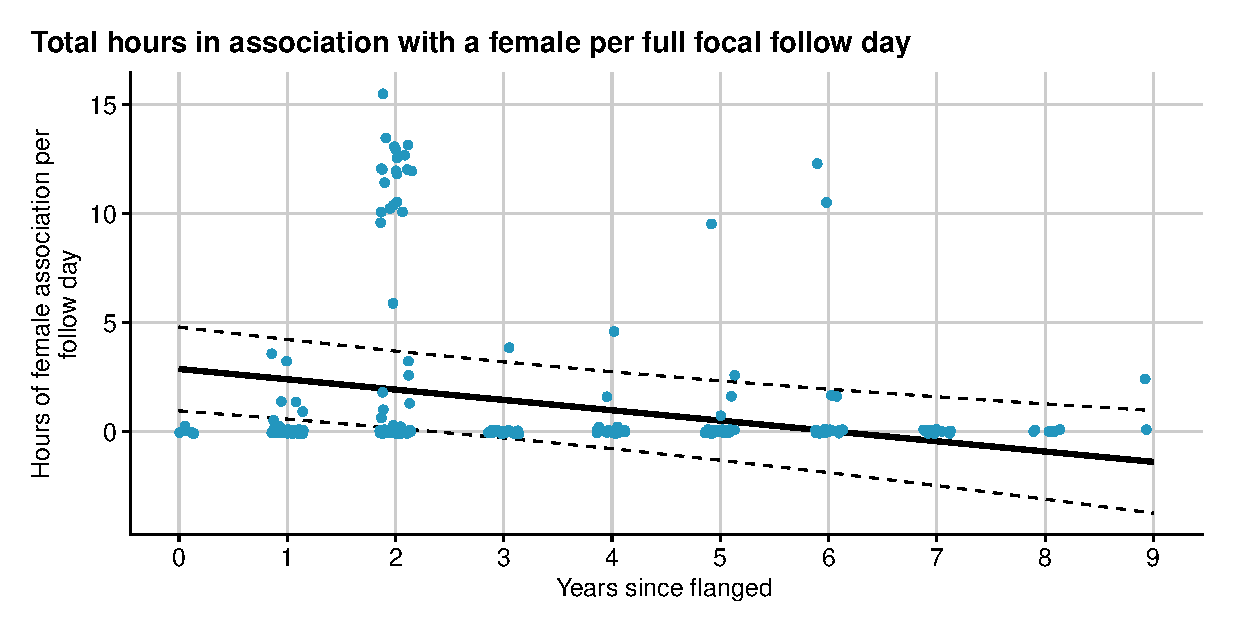
\includegraphics[width=1\linewidth]{Chapter4/Figs/FemAssocPlot.eps}
\caption{Examination of the impacts of ecological and social factors on the total hours of female association per full focal follow day. The plot presents the relationship between the number of years since the orangutan was first produced a long call and the total number of hours per follow day they spent within 50m of a female. The lines with dashed boundaries show the predicted response and confidence intervals generated from the mixed model results.}
\label{fig:Female Association Dynamics with Flanged Males as a function of Age in Tuanan Field Station}
\end{figure}

\subsection{Impact of relative age on long call behaviour and composition}

To examine the impacts of age since flanging, I used three more linear mixed effects models. I conducted two Poisson GLMMs to investigate the number of long calls per follow day and the average number of pulses per long call (Table 4.3).

Model 4 (Table 4.3) focused on the number of long calls per follow day. FAI had a positive impact on the number of long calls, being marginally significant (Estimate = 0.079, p-value = 0.046). However, all other fixed effects, did not have a signficant effect on the number of long calls produced per day (Years since flanged: Estimate = -0.009, p-value = 0.857; hours in female association: Estimate = -0.176, p-value = 0.081; total hours of rain: Estimate = -0.003, p-value = 0.439; number of long calls heard: Estimate = 0.014, p-value = 0.280).

Model 5 (Table 4.3) examined the average number of pulses per long call (including long call duration as an offset term). I found a strong negative relationship between Year since flanged and the average number of pulses per long call, which was statistically significant (Fig. 4.3., Estimate = -0.0821, p-value < 0.001). The number of long calls heard (LCH) also showed a negative association with the number of pulses per produced long call and was also statistically significant (Estimate = -0.01986, p-value = 0.02488).
As seen in Model 4, hours of female association, FAI and total rain were not significant predictors, with p-values of 0.110 and 0.958, respectively.

\begin{table}
    \centering
    \resizebox{\textwidth}{!}{%
\begin{tabular}{l l r r r r}
\hline 
\multirow{1}{*}{\textit{Response}} &  \multirow{1}{*}{\textit{Fixed effects}} & \multirow{1}{*}{\textit{Estimate}} & \multirow{1}{*}{\textit{Std. Error}} & \multirow{1}{*}{\textit{z}} & \multirow{1}{*}{\textit{Pr(>|z|)}}\\ 
\hline
\textbf{4. Number of long calls per follow day} & \textbf{Intercept} & \textbf{-1.488} & \textbf{0.334} & \textbf{-4.458} & \textbf{< 0.001} \\
& Years Since Flanged & -0.009 & 0.048 & -0.180 & 0.857 \\
\textit{Poisson GLMM}, \textit{N = 110} & \textbf{FAI} & \textbf{0.079} & \textbf{0.039} & \textbf{2.005} & \textbf{0.046} \\
\textit{Offset(ObsTime)} & FemAssocH & -0.176 & 0.101 & -1.743 & 0.081 \\
$\Delta$ AIC = 328.158  & Total Rainfall (h) & -0.003 & 0.004 & -0.773 & 0.439 \\
& Long Calls Heard & 0.014 & 0.013 & 1.081 & 0.280 \\
\cline{2-6}
& \textit{Random effects} & & & \textit{Variance} & \textit{Std. dev.}\\
\cline{2-6} 
& Name & & & 0.179 & 0.423 \\
& Month:Name & & & < 0.001 & < 0.001 \\
& Year:Month:Name & & & 0.205 & 0.453 \\
\hline 
\textbf{5. Average number of pulses per long call} & \textbf{Intercept} & \textbf{0.767} & \textbf{0.136} & \textbf{5.636} & \textbf{< 0.001} \\
 & \textbf{Years Since Flanged} & \textbf{-0.082} & \textbf{0.023} & \textbf{-3.521} & \textbf{< 0.001} \\
\textit{Poisson GLMM}, \textit{N = 102} & FAI & 0.008 & 0.020 & 0.404 & 0.686 \\
& FemAssocH & -0.103 & 0.064 & -1.598 & 0.110 \\
$\Delta$ AIC = 459.604 & Total Rainfall (h) & -0.001 & 0.002 & -0.052 & 0.959 \\
& \textbf{Long Calls Heard} & \textbf{-0.020} & \textbf{0.009} & \textbf{-2.243} & \textbf{0.025} \\
\cline{2-6}
& \textit{Random effects} & & & \textit{Variance} & \textit{Std. dev.}\\
\cline{2-6} 
& Name & & & 0.014 & 0.120 \\
& Month:Name & & & < 0.001 & < 0.001 \\
& Year:Month:Name & & & 0.048 & 0.219 \\
\hline 
\end{tabular}

}
    \caption{Results of the Poisson mixed-effects models examining the impacts of years since flanged, Fruit Availability Index, total hours of rainfall, female association (hours), and long calls heard on the number of long calls, and number of long call pulses per full focal follow day. These models include random effects for individual ID nested within Year and Month.
    Formula used was: \(Response \sim YearsSinceFlanged + FAI + FemAssocH + TotalRainfall.h + LCH + (1 |Name/Year/Month)\) }
\end{table}
Finally, Model 6 (Table 4.4.) examined the relationships of the fixed effect on average long call duration. This model found a significant negative relationship between the number of years since flanging and average long call duration, with individuals who have been flanged longer producing significantly shorter long calls (Fig. 4.3., Estimate = -2.6961, p-value = 0.011). However, all other fixed effects did not have a statistically significant impact on average long call duration (FAI: Estimate = 0.2879, p-value = 0.7192; FemAssocH: Estimate = -0.9427, p-value = 0.7721; total hours of rainfall: Estimate = -0.1591, p-value = 0.2031; long calls heard: Estimate = -0.3899, p-value = 0.4146).
\begin{table}
    \centering
    \resizebox{\textwidth}{!}{%
\begin{tabular}{l l r r r r}
\hline 
\multirow{1}{*}{\textit{Response}} &  \multirow{1}{*}{\textit{Fixed effects}} & \multirow{1}{*}{\textit{Estimate}} & \multirow{1}{*}{\textit{Std. Error}} & \multirow{1}{*}{\textit{z}} & \multirow{1}{*}{\textit{Pr(>|z|)}}\\ 
\hline
\textbf{6. Average long call duration per follow day} & \textbf{Intercept} & \textbf{49.584} & \textbf{5.796} & \textbf{8.555} & \textbf{< 0.001} \\
& \textbf{Years Since Flanged} & \textbf{-2.696} & \textbf{1.061} & \textbf{-2.541} & \textbf{0.011} \\
\textit{Gaussian GLMM}, \textit{N = 64} & FAI & 0.288 & 0.801 & 0.360 & 0.719 \\
& FemAssocH & -0.943 & 3.254 & -0.290 & 0.772 \\
$\Delta$ AIC = 455.311  & Total Rainfall (h) & -0.159 & 0.125 & -1.273 & 0.203 \\
& Long Calls Heard & -0.390 & 0.478 & -0.816 & 0.415 \\
\cline{2-6}
& \textit{Random effects} & & & \textit{Variance} & \textit{Std. dev.}\\
\cline{2-6} 
& Name & & & 20.5 & 4.528 \\
& Residual & & & 143.8 & 11.992 \\
\hline 
\end{tabular}
}
    \caption{Results of the Gaussian mixed-effects model examining the impacts of years since flanged, Fruit Availability Index, total hours of rainfall, females association (hours) and long calls heard on the average duration of long calls made per full focal follow day. This model includes a random effect for individual ID.
    Formula used was: \(Response \sim YearsSinceFlanged + FAI + FemAssocH + TotalRainfall.h + LCH + (1 |Name/Year/Month)\) }
\end{table}






\begin{figure}
\centering
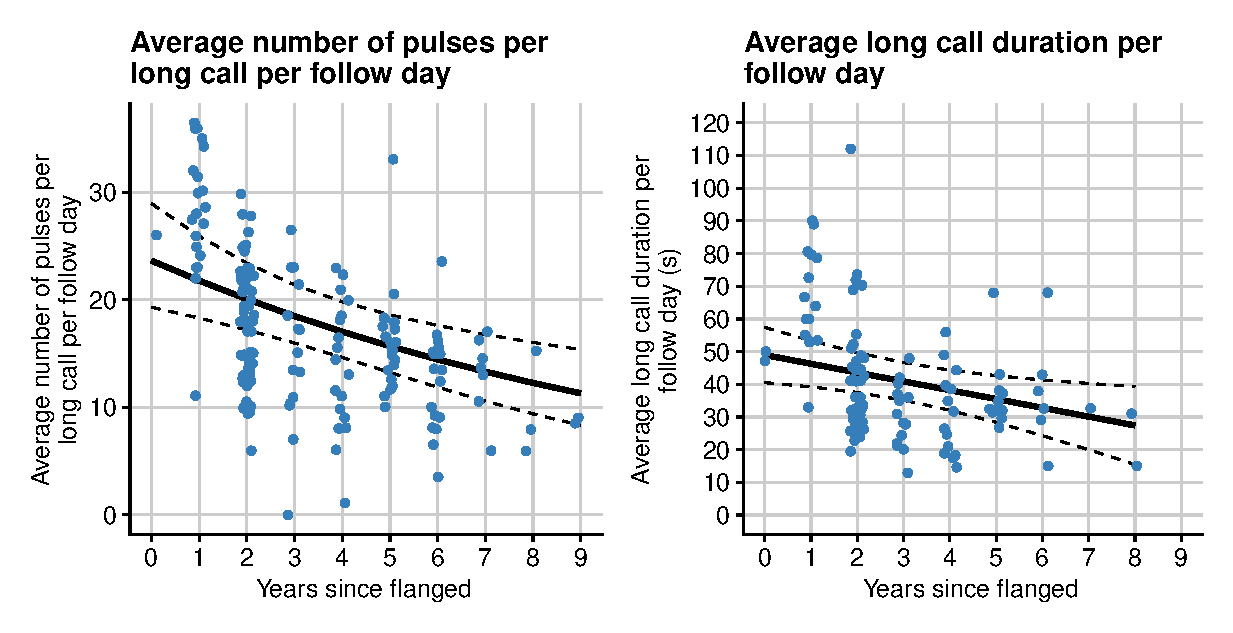
\includegraphics[width=1\linewidth]{Chapter4/Figs/combined_plot.eps}
\caption{Impacts of ageing on long call composition and duration. The left plot shows how the average number of pulses changes according to relative age since flanging. The right plot shows how average long call duration per day is impacted by relative age since flanging.}
\label{fig:Flanged_male_association_between_Suaq_and_Tuanan}
\end{figure}



\section{Discussion}

The combination of semi-social social structure, unflanged ranging behaviour, and bimature male physiology makes examining the impact of age on sociality in wild flanged male orangutans particularly challenging. However, despite these limitations and our small individual sample size, this study has found a number of age-related changes in female association and long call behaviour.

\subsection{Impacts of age on female association behaviour}

Contrary to my hypothesis, this study did not find a change in the number of females associated with per follow day as a function of age after flanging. However, I did find that older individuals spend less time in association with a female per follow day. Male orangutans are the dominant sex, so these findings are broadly in line with observations from other great apes, suggesting that older individuals of the dominant sex spend more time alone as they age \citep{Rosati.2020}.  Furthermore, these trends are found in a variety of old world monkeys, including grey Langurs (\textit{Semnopithecus entellus}), rhesus macaques (\textit{Macaca mulatta}) and barbary macaques (\textit{Macaca sylvanus}) \citep{Hrdy.1976, Corr.2003, Almeling.2017, Siracusa.2022}.

 As previously mentioned, several theories attempt to explain the increased inclination for solitude in older primates as they age. The Socioemotional Selectivity Theory (SST) posits that as humans recognise their limited time remaining, they prioritise emotionally meaningful interactions, leading to a reduced desire for broad social networks which results in increased time spent alone \citep{Carstensen.2021}. However, this theory hinges on the individual being a) aware of their own mortality and b) able to imagine the future in an abstract sense. There is limited evidence that chimpanzees show some of the key behavioural signatures of SST, including a positive interaction bias with age, increased proportion of their social interactions being mutually beneficial and a smaller social network \citep{Rosati.2020}. As such, these evolutionary origins may be present in orangutans beyond a cost-benefit analysis of the risks of engaging in social behaviour imposed by age-related degradation of bone and muscle strength that may be shared more widely across primates \citep{González.2023}.

One of the limitations of the study is that even though I observed a decrease in female association time as flanged males continue to age, I was not able to discern whether this trend is attributed to solely age-related social selectivity on the part of the flanged male, or whether the decrease in association time was driven by female preferences. Female association time per follow day is driven in part by consortships, where females travel with flanged males for a few days, mating frequently \citep{O'Connell.2020}. As such, these results may suggest that females are less likely to enter consortships with older males, or they are considerably shorter in duration. This decrease in association time may also be driven in part by visual clues of age related degradation in appearance (\citep{Jolly.2009}, Chapter 3). These causes are not mutually exclusive as both male selectivity and female preference might both influence association dynamics. Disentangling the ultimate causes will require a longer term analysis of which party initiates the termination of interactions, and how frequently each party approaches or moves away from the other.

One limitation of this study is the omission of male-male interactions in the data set. While encounters between flanged males are typically antagonistic in nature, influenced by competition for resources and mates, they can display tolerance towards unflanged males \citep{Setia.2008}. Incorporating these interactions might reveal whether older flanged males exhibit decreasing aggression with age or show increased tolerance towards unflanged counterparts. Understanding such dynamics would provide a more holistic view of how age influences male orangutan sociality and could potentially refine or challenge my current findings, and add to the evidence that the evolutionary origins of SST can be found in other great apes.

However, as the number of females in association per follow day was not significantly different, these findings also suggest that females do not selectively choose to approach younger flanged males based off their long calls, despite having differences in composition over time. This may be in part due to limitations of the data set, this study focused entirely on individuals whose identity was known before undergoing the morphological change to a flanged male to control for age-linked social biases due to development arrest. As such, the "oldest" individual was only +9 years from production of their first long call, which may not be old enough to capture the full range of behavioural shifts that occur as flanged males age. 

The negative relationship between fruit availability and number of fertile females in association per follow day were also interesting, particularly given that long call frequency appears to increase during this time. I hypothesise this may be a strategy of energy maximisation on the part of females: during periods of high fruit availability fertile females may have reduced necessity for direct association for resource access and hence less willing to move toward long calls produced by flanged males. As such, the increase in flanged male long calls during these times may be a coping mechanism to reduced female receptivity. However, it has been previously hypothesised that periods of high fruit availability may be when fertile females are more available \citep{Spillmann.2016}. Females spend a considerable amount of time and energy lactating, and need to recover this deficit before being able to conceive again \citep{Knott.2008dtq}. Given the calorific requirements, it's more likely this will fall during periods of high fruit availability,  and as females conceal their fertility status, flanged males may increase their long call frequency per day during this period lacking other environmental clues (which was observed in Model 4). This may be because females are more selective during this period and opportunistically approach a smaller number of flanged males based on their long call, and is backed up by the fact that the random effect of individual identity contributed substantially to the variance within this model. However, as this study pooled individual results I was not able to find significant differences between individuals, and a within-individual between-individual analysis may be better able to diagnose the impact of individual identity on fertile female associative behaviour.

\subsection{Impacts of age on long call behaviour}

This study also found significant relationships between the relative age of the flanged male and their long call behaviour. Specifically, older flanged males seem to produce shorter long calls and fewer pulses during these vocalisations. 

There are two possible non-mutually exclusive causes for these observed trends, the first of which is that the change in long call composition over time is driven by social factors. 

Longs calls serve a number of purposes for the producers: they establish individual identity, they are used as a form of confrontational assessment between flanged males, and are used to attract females \citep{Mitani.1985, Spillmann.2016, Setia.2007}. These calls are also highly context-dependent and can be produced either spontaneously or in response to a specific cue, such as a tree falling or hearing another long call \citep{Spillmann.2010}. These contexts impact the reaction of females to the long calls, as female ranging responses to reactive long calls are significantly lower than ranging towards spontaneously produced long calls \citep{Spillmann.2016}. Notably, reactive long calls generally contain a greater number of pulses compared to spontaneous long calls \citep{Spillmann.2016}. Recently flanged males may react more frequently or more intensely to cues in order to establish their presence in an area, however once their home range is established, their reaction to the cues may be slightly reduced. This hypothesis is backed up when considering the noticeable peak in the number of pulses and duration of long calls observed during the first two years post-flanging (Fig. 4.3.). Additionally, the change in the number of pulses could be due to the impact of age-related shifts in emotional reactivity which has been observed in humans \citep{Grühn.2016}. In males, these changes may correlate with a decrease in circulating testosterone levels during ageing, decreasing aggression rates \citep{Book.2001}. These social factors are not mutually exclusive and the observed effect could be due to both of these factors. Untangling the impact of emotional reactivity in ageing flanged males would likely require lengthy long call data sets using acoustic location systems to examine the separate impacts of distance, age, local dominance, and long call triggers which is sadly beyond the scope of the current study \citep{Spillmann.2016}. 

However, it is also possible that these shifts in long call composition and duration are influenced by the physiological and energetic constraints associated with ageing. Vocalisations in many primates undergo changes as they age, with potential reasons ranging from muscle degeneration, altered hormone levels, to reduced lung capacity, which could affect the strength and duration of calls \citep{Ey.2007, Pistorio.2006, Inoue.1988}. For example, in humans, increased age in adults synergistically increases changes in vocal jitter caused by poor body condition \citep{Ramig.1983}. Additionally, ageing affects the quality and strength of voice due to changes in the vocal cords and respiratory system, as older individuals experience reductions in total lung capacity as they age \citep{Teramoto.1999}. As flanged males age, the energetic costs of producing these calls may become substantial, and older males might be economising their energy expenditure in light of decreasing physical robustness or metabolic changes.

The distinction between these two hypotheses, the social determinants vs. physiological constraints, could be achieved through a combination of detailed observational studies and physiological measurements. Monitoring older flanged males in varying social contexts, such as when new males enter their territory or during periods of increased female fertility, could provide information on the social implications of their calls \citep{Spillmann.2016, Hayward.2018}. Concurrently, employing non-invasive techniques on captive orangutans to assess their respiratory functions, muscle strength, and overall energy metabolism over time can offer a clearer picture of the physiological costs of their vocal behaviour. Combining these methodologies will not only facilitate a comprehensive understanding of age-related changes in vocal behaviour but will also help draw broader inferences about the life histories and social dynamics of orangutans and other great apes.

My finding that long call rates per follow day increase with FAI stand in contrast to previous studies of long call behaviour, which have not found a correlation between fruit availability and long call rates in the same field site (with a different data set) \citep{Spillmann.2016}. Fruit availability in Tuanan follows a similar pattern each year, with the "lean" season between April and September, however the total fruit availability between years can vary significantly, despite lacking the community wide masting events seen in lowland dipterocarp forests of the same region (Fig. 3.3, \citep{Harrison.2016}). As previously mentioned, I suggest this may be due to the increased availability of females, and given that female fertility is concealed, this ecological correlation may be the best approximation males have for the presence of fertile females. The interplay between foraging and socio-sexual signalling can be complex, and may also involve indirect effects. Future studies, ideally incorporating larger sample sizes and diverse environmental contexts, would be instrumental in deciphering the intricate dynamics that underpin these behaviours.

\subsection{Limitations}
Caution should be taken when interpreting the behaviour of 6 individuals to draw species-wide conclusions, particularly since these individuals inhabit the same habitat, and these trends are likely to differ according to the local dominance hierarchy and stability of the area. Additionally, this study did not examine changes in frequency or amplitude, which may also be indicative of changes in long call behaviour detectable to females and other males, and may be indicative of degrading body condition. Finally, as previously mentioned this study pooled individual measures therefore it was not able to detect changes between individuals beyond the random effect structure. 

\nomenclature[z-SST]{SST}{Socioemotional Selectivity Theory}